\documentclass[12pt]{article}
\usepackage{amsmath}
\usepackage{amsfonts}
\usepackage{fancyhdr}
\usepackage{titlesec}
\usepackage[margin=1in]{geometry}
\usepackage{siunitx}
\usepackage{booktabs}
\usepackage{graphicx}

\pagestyle{fancy}
\lhead{} 
\chead{} 
\rhead{\thepage} 
\lfoot{} 
\cfoot{} 
\rfoot{} 
\renewcommand{\headrulewidth}{0pt} 
\renewcommand{\footrulewidth}{0pt} 
%\titleformat{\section}[block]{\Large\bfseries\filcenter}{}{1em}{}
%\titleformat{\subsection}[block]{\large\bfseries\filcenter}{}{1em}{}
%To make sure we actually have header 0.5in away from top edge
%12pt is one-sixth of an inch. Subtract this from 0.5in to get headsep value
\setlength\headsep{0.333in}
\pagestyle{fancy}
\linespread{1.4}

\newcommand{\boldrule}{\rule{\linewidth}{2pt}} % Draws a thick line


\graphicspath{{Graphics/}}

\begin{document}

\thispagestyle{empty}
\newpage
\vspace*{3cm}
\begin{center}
%Lab title goes here
{\Huge EE 648 -- VLSI Design\\[.5cm]
Binary Coded Hexadecimal for a 7 Segment Display}
\end{center}
\vspace{5mm}
\boldrule\\
\begin{center}

\includegraphics{uaflogo.png}\\[.5cm]
\boldrule\\[3cm]
{\Large
\textsc{Ryker Dial}\\
\textsc{Cody Gossel}\\
\textsc{Zach Krehlik}\\[1cm]
May 1, 2015
}
\end{center}



\newpage

\thispagestyle{empty}
\tableofcontents

\newpage

\setcounter{page}{1}

%Rest of report goes here

\begin{figure}[h]
	\centering
	\label{fig:TopLevelCkt}
	\caption{Circuit top level layout}
	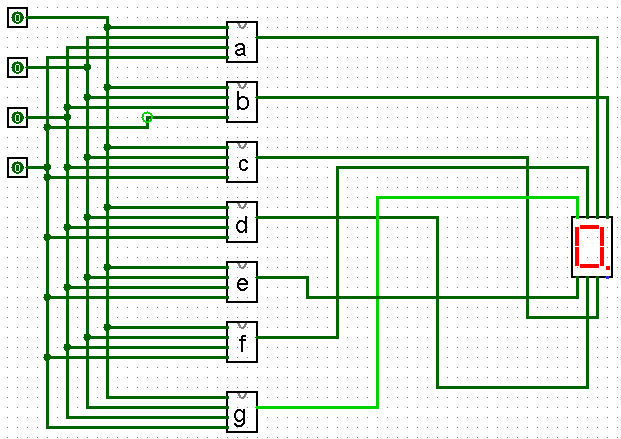
\includegraphics[scale=.8]{topLevelLogicCkt.png}
\end{figure}









\end{document}
